\documentclass[a4paper]{article}
\usepackage{titling}
\usepackage{authblk}
\usepackage{fancyhdr}
\usepackage{url}
\usepackage{hyperref}
\usepackage{rsc}
\usepackage{siunitx}
\usepackage{graphicx}
\usepackage{listings}
\usepackage{color}
\usepackage{tikz}
\usetikzlibrary{shapes,arrows}


\definecolor{dkgreen}{rgb}{0,0.6,0}
\definecolor{gray}{rgb}{0.5,0.5,0.5}
\definecolor{mauve}{rgb}{0.58,0,0.82}

\lstset{frame=tb,
  language=Python,
  aboveskip=3mm,
  belowskip=3mm,
  showstringspaces=false,
  columns=flexible,
  basicstyle={\ttfamily},
  numbers=none,
  numberstyle=\tiny\color{gray},
  keywordstyle=\color{blue},
  commentstyle=\color{dkgreen},
  stringstyle=\color{mauve},
  breaklines=true,
  breakatwhitespace=true,
  tabsize=3
}
\DeclareSIUnit\Fahrenheit{\degree F}

\title{Data analysis with Python}
\author[1]{Dr Benjamin J. Morgan}
\author[1,2]{Dr Andrew R. McCluskey}
\affil[1]{Department of Chemistry, University of Bath, email: b.j.morgan@bath.ac.uk}
\affil[2]{Diamond Light Source, email: andrew.mccluskey@diamond.ac.uk}
\setcounter{Maxaffil}{0}
\renewcommand\Affilfont{\itshape\small}

\pagestyle{fancy}
\fancyhf{}
\rhead{CH40208}
\lhead{\thetitle}
\rfoot{\thepage}

\begin{document}
\maketitle

\section*{Aim}
Data analysis is an incredibly important skill in chemistry, however, it is often overlooked. 
In this exercise, you will get an introduction to using Python to fit experimental data, see how model-dependent analysis works in a simple system, and write a Markov chain Monte Carlo algorithm to quantify the inverse uncertainty in your model.
The particular application in this work is the analysis of an IR spectra from a mixture of organic species, however, hopefully you will recognise that the methods used herein are generalisable.

\section{Reading in and plotting experimental data}
You have been tasked with determining the relative composition of a mixture of two organic species; namely toluene and benzyl alcohol (Figure~\ref{fig:mole}). 
To do this, you have measured the infrared spectra of the mixture and obtained (from the NIST Chemistry WebBook) the model spectra of the two species in isolation, these can be found in the `IR spectra' folder on Moodle. 
If you download and open the files in the Jupyter Notebook file viewer, you can see the structure of the files. 
You should note that the model datasets (\texttt{benzyl\_alcohol.csv} and \texttt{toluene.csv}) consist of two columns; wavenumber ($\bar{\nu}$) and transmittance ($T$), while the measured experimental data (\texttt{mixture.csv}) has a third column that describes the uncertainty in the transmittance. 
%
\begin{figure}[t]
  \centering
  \includegraphics[width=0.5\textwidth]{drawing}
  \label{fig:mole}
  \caption{The organic species in the mixture.}
  \end{figure}
%
\vspace{\baselineskip}
\begin{center}
	\noindent\fbox{%
	    \begin{minipage}{0.9\textwidth}%
	        \vspace{0.15\baselineskip}
			\subsubsection*{Objective 1}
          \begin{itemize}
            \item {Read in the two model datasets, plot them separately using \texttt{matplotlib} including axis labels}
            \item {Read in the experimental dataset, including the third column. Then investigate how this may be plotted using the \texttt{plt.errorbar} functionality} 
          \end{itemize}
          \textbf{Hint}: Googling `matplotlib errorbar' offers some useful instructions on how to use this function, or you can read the documentation with \texttt{plt.errorbar?} in the Jupyter Notebook.
	    \end{minipage}
	}
\end{center}

Having plotted each of the three datasets (the two models and the experimental), you should be able to identify features present in the experimental data that match those in the models. 
Such as the large feature in the toluene model data, that we can see in the experiment at around \SI{3000}{\per\centi\meter}, and then at higher energy (higher wavenumber), there is a broad feature in the benzyl alcohol data, between \SIrange{3250}{3750}{\per\centi\meter}, that can be found in the experimental data. 

\section{Fitting}
You will have hopefully encoutered fitting to data before, for example fitting a line of best fit to some datapoints.
This is shown in Figure~\ref{fig:plot}, where the blue dots are some discrete datapoints and the orange line is the line of best fit. 
In order to determine this line of best fit, we have a metric that we want to minimise that represents the difference between the data and the model (the line).
This metric is shown in the lower plot, which is the square residual, calculated as the difference between the data point and the position on the $y$-axis of the line at the same $x$-axis position as the data point, squared.
The purpose for the squaring is to put a heavier emphasis on the outlining datapoints, where the difference is large. 
We can collapse these values for the individual datapoints down into a single value by taking the sum of these square residuals.
This goodness-of-fit metric is referred to as the $\chi^2$-value for the fit, the closer the $\chi^2$ is to zero, the better the agreement between our model and data. 
%
\begin{figure}[t]
  \centering
  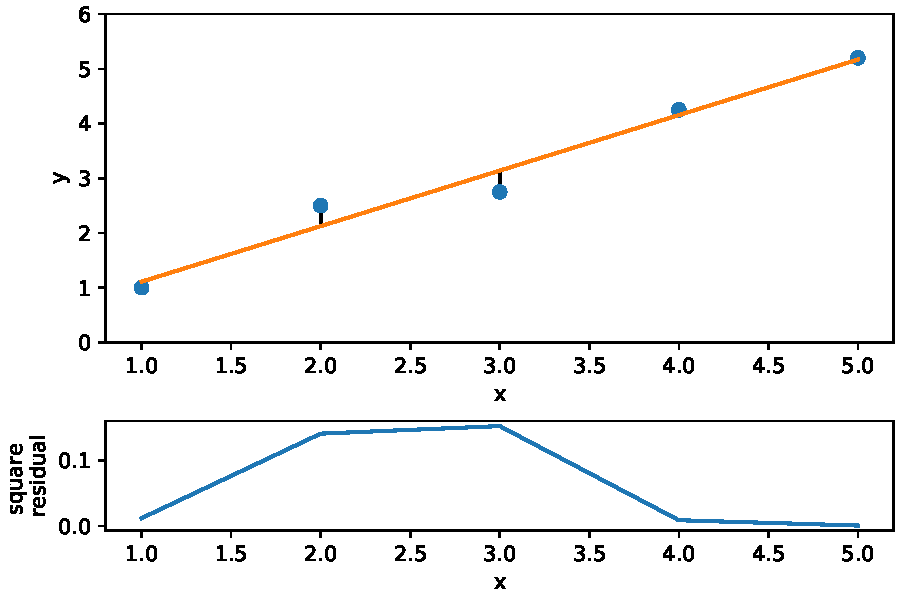
\includegraphics[width=0.8\textwidth]{residual}
  \label{fig:plot}
  \caption{A line of best fit through some datapoints and the squared residuals of the fit.}
  \end{figure}
%

\section{Interpolation}
From your earlier plots, you may note that the values of wavenumber that the spectra have been measured over is not the same between the three datasets, this can be clearly seen by printing the wavenumber range for each of the three datasets. 
In order to determine the $\chi^2$-value between our model (outlined later) and the data (the mixture), it is necessary that the positions on the $x$-axis for the two are the same, and since our model will be created from mixing the toluene and benzyl alcohol spectra we will need to normalise these $x$-axes. 
This means that interpolation is necessary. 

Interpolation is where we determine new data points within the range of a discrete set of known points. 
Essentially we use what we know about the $x$- and $y$-values and guess at the $y$-values of the different set of $x$ values. 
It is important that the new range of $x$-values is from within the existing range, or else we would be extrapolating (which is often unscientific). 
For the data that you are using, the experimental data lies within the range of the other two datasets, and therefore we will use the wavenumber $x$-values from the experimental dataset and interpolate values for the model data.

To interpolate new $y$-values for the two models, we will use the \texttt{np.interp} function, the documentation for this can be found online (\url{https://docs.scipy.org/doc/numpy/reference/generated/numpy.interp.html}) or by using the \texttt{?} command in the Jupyter Notebook.
Note that this function takes three arguments, in the documentation these are called \texttt{x} which is the new $x$-axis that values should be interpolated for, \texttt{xp} which is the old $x$-axis values, and \texttt{fp} which is the old $y$-axis values. 
This function will return a new set of $y$-axis values, which you should store in a suitably named variable. 

\vspace{\baselineskip}
\begin{center}
	\noindent\fbox{%
	    \begin{minipage}{0.9\textwidth}%
	        \vspace{0.15\baselineskip}
			\subsubsection*{Objective 2}
          \begin{itemize}
            \item {By evaluating the minimum and maximum of each dataset (using the \texttt{np.min} and \texttt{np.max} functions), prove to yourself that the experimental data lays within the model data on the $x$-axis} 
            \item {Create a new variable called \texttt{optimisation\_x} which is the range of $x$-values to be interpolated over (make it equal to the wavenumebr values for the mixture data)}
            \item {Using \texttt{np.interp}, interpolate the toluene and benzyl alcohol data within the values of wavenumber for the mixture}
            \item {Plot the interpolated data to ensure that the interpolation looks similar to the original data}
          \end{itemize}
	    \end{minipage}
	}
\end{center}

\section{Fitting real data}
In the straight line example in Figure~\ref{fig:plot}, we were not working with ``real'' data as there was no uncertainty on the value of the data points. 
However, if we compare the slope of the straight line in Figure~\ref{fig:plot} with that in Figure~\ref{fig:plot_err} (once we consider uncertainty), there is a change from 1.015 to 1.037 -- a small but significant change. 
In order to consider the uncertainty, there is a slight modification to the $\chi^2$-value calculation, where the square residual is divided by the uncertainty at the point, 
%
\begin{equation}
  \chi^2 = \sum_{i=0}^{N}\bigg[{\frac{y_{\text{model, i}} - y_{\text{exp, i}}}{\text{d}y_{\text{exp, i}}}\bigg]^2},
  \label{equ:chi}
\end{equation}
%
where, $y_{\text{model, i}}(c)$ is the model (the straight line), $y_{\text{exp, i}}$ is the experimental data point, $\text{d}y_{\text{exp, i}}$ is the uncertainty in the experimental data point, and $N$ is the number of points in the dataset.
%
\begin{figure}[t]
  \centering
  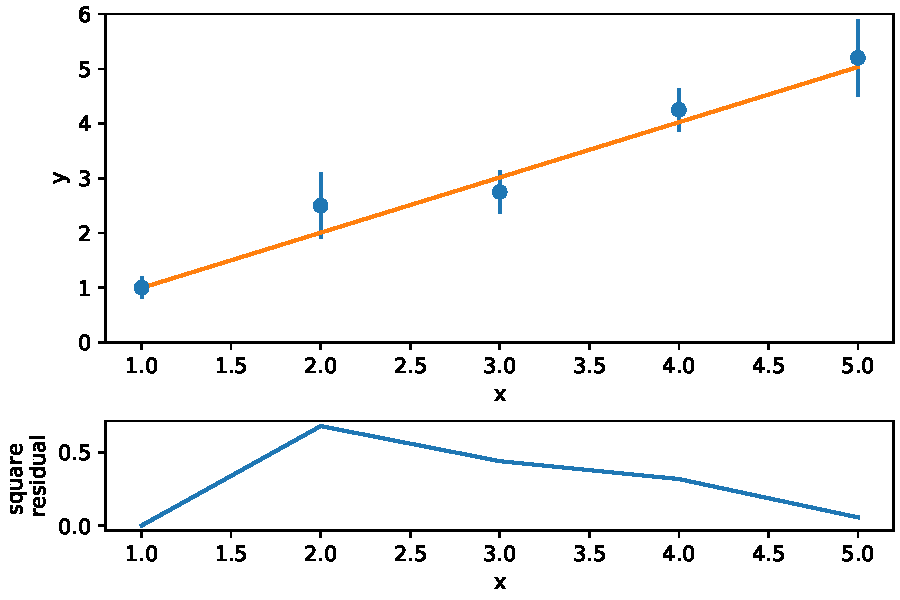
\includegraphics[width=0.8\textwidth]{residual_err}
  \label{fig:plot_err}
  \caption{A line of best fit through some datapoints with uncertainty and the squared residuals of the fit.}
  \end{figure}
%

Now that all three models have the same $x$-axis and we are aware of how to fit real data, it is possible to begin the procedure of fitting the experimental data to determine the composition of the mixture. 
The function that we will be fitting is the following, 
%
\begin{equation}
  T_{\text{mixture}} = c T_{1} + (1 - c)T_{2},
  \label{equ:model}
\end{equation}
%
where $1$ and $2$ indicate toluene and benzyl alcohol respectively, and $c$ is the fractional composition of toluene (therefore, $1-c$ is the fractional composition of benzyl alcohol as we assume that this is only a two component mixture). 

\vspace{\baselineskip}
\begin{center}
	\noindent\fbox{%
	    \begin{minipage}{0.9\textwidth}%
	        \vspace{0.15\baselineskip}
			\subsubsection*{Objective 3}
          \begin{itemize}
            \item {Write a function that evaluates Equation~\ref{equ:model}, remember to include a docstring}
            \item {Test the function by using it to plot the spectra that would result from a 50:50 mixture of the two components against the experimental mixture data}
          \end{itemize}
	    \end{minipage}
	}
\end{center}

A 50:50 mixture of the two components doesn't do a very good job of modeling the data, therefore we should optimise this value.
We can optimise this value by finding the value that minimises the $\chi^2$-value, which can be achieved using the \texttt{scipy.optimize} function that was introduced in week 3 called \texttt{minimize}. 

\vspace{\baselineskip}
\begin{center}
	\noindent\fbox{%
	    \begin{minipage}{0.9\textwidth}%
	        \vspace{0.15\baselineskip}
			\subsubsection*{Objective 4}
          \begin{itemize}
            \item {Write another function that will evaluate the value of $\chi^2$ for a given $c$, remember to include a docstring}
            \item {Recalling the use of \texttt{scipy.optimize.minimize}, try and determine the optimum value to minimise the difference between the experiment and the model}
            \item {Store the result of the optimisation and plot the model with the optimised value of $c$ on top of the experimental data to allow you to visually observe the similarity}
          \end{itemize}
	    \end{minipage}
	}
\end{center}

\section{Markov chain Monte Carlo}
If we think of uncertainties as representing a distribution of possible values for a data point, for example if the measurement was conducted 10 times, you would get values within this uncertainty. 
Therefore, we can imagine that if the data in Figure~\ref{fig:plot} was collected 10 times, there would be some distribution of values, and if we independently fit a straightline to each of these 10 data collections, we would get slightly different values for the slope. 
This distribution of values for the slope, leads to what is referred to as the \emph{inverse uncertainty} which is the uncertainty on a model's parameter that arises due to uncertainty in the measurement that is propagated through the fitting of the model. 
There are a number of methods that we can use to quantify this inverse uncertainty, including the Markov chain Monte Carlo (MCMC) methods introduced here. 

A Markov chain is a \emph{random-walk} through a series of numbers while the Monte Carlo part implies that we use probability to determine if a \emph{transition} is possible.
In MCMC we start with an initial guess for a variable, which can be taken from a traditional minimisation such as that used in \texttt{minimize} and then perturb it by some random amount. 
This random amount is typically obtained based on a step size change with respect to the value of the variable, 
%
\begin{lstlisting}
  perturbation = step\_size * np.random.random() * c,
\end{lstlisting}
%
where, \texttt{c} is the variable to be perturbed.
We then determine if this random perturbation has improved the agreement to the data (the $\chi^2$-value) or not. 
If it has, we \textbf{accept} this new value for our variable and perform another perturbation. 
If the perturbation does not improve agreement to the data, the new value is \textbf{not} immediately rejected, rather it is only rejected if the probability of this \emph{transition} ($p$) is less than some random number from 0 to 1. 
The probability is found by, 
%
\begin{equation}
  p = \exp{\bigg(\frac{-\chi^2_{\text{new}} + \chi^2}{2}\bigg)},
  \label{equ:prob}
\end{equation}
%
where, $\chi^2$ is the original goodness-of-fit value and $\chi^2_{\text{new}}$ is the goodness of fit after the perturbation. 
This means that it is possible for the agreement to get worse overtime, however, the amount by which it can get worse is affected by Equation~\ref{equ:prob}. 
Due to the application of Equation~\ref{equ:prob}, the only values of $\chi^2$ that may be accessed by the Markov chain (these random perturbations on our value) are those that are statistically feasible given the uncertainty on the experimental measurements. 

The algorithm for a typical MCMC sampling process is as follows (this is also described with a flow diagram in Figure~\ref{fig:flow}), 
\begin{enumerate}
  \item {Create an empty list called \texttt{accepted}}
  \item {Evaluate $\chi^2$ for the initial guess of $c$, typically this initial guess would be obtained from a standard optimisation}
  \item {Perturb $c$}
  \item {Calculate $\chi^2_{\text{new}}$ for the new value of $c$}
  \item {Determine the probability of this \emph{transition}, from Equation~\ref{equ:prob}}
  \item {Check if $p \ge n$ where $n$ is a random number from 0 to 1 (this can be obtained from \texttt{np.random.random()}, note that if the new $\chi^2$ is less than the old one then $p > 1$ and therefore this is always accepted}
  \item {If yes, update values of $c$ and $\chi^2$}
  \item {Go to 3 and repeat until the desired number of iterations has been achieved}
\end{enumerate}


% Define block styles
\tikzstyle{decision} = [diamond, draw, fill=blue!20, 
    text width=4.5em, text badly centered, node distance=3cm, inner sep=0pt]
\tikzstyle{block} = [rectangle, draw, fill=blue!20, 
    text width=5em, text centered, rounded corners, minimum height=4em]
\tikzstyle{line} = [draw, -latex']
\tikzstyle{cloud} = [draw, ellipse,fill=red!20, node distance=3cm,
    minimum height=2em]
%
\begin{figure}[t]
  \centering

\begin{tikzpicture}[node distance = 4cm, auto]
    % Place nodes
    \node [block] (init) {initialize empty list};
    \node [block, right of=init] (chi) {calculate $\chi^2$ for initial guess};
    \node [block, below of=chi] (perturb) {add some random noise to the variable};
    \node [block, below of=perturb] (newchi) {calculate $\chi^2$ for perturbed guess};
    \node [block, below of=newchi] (prob) {calculate the probability};
    \node [block, left of=prob] (decide) {get $n$ ($n$ is a random number)};
    \node [block, left of=perturb] (store) {store variable in list and update variable};
    \node [block, left of=store, node distance=5.2cm] (exit) {exit};
    % Draw edges
    \path [line] (init) -- (chi);
    \path [line] (chi) -- (perturb);
    \path [line] (perturb) -- (newchi);
    \path [line] (newchi) -- (prob);
    \path [line] (prob) -- (decide);
    \path [line] (store) -- (perturb);
    \path [line] (decide) -- node [near end] {if $p \ge n$} (store);
    \path [line] (decide) -- node {else} (perturb);
    \path [line] (store) -- node [align=center] {if max iterations \\ is reached} (exit);
    %\path [line] (decide) -| node [near start] {yes} (update);
    %\path [line] (update) |- (identify);
    %\path [line] (decide) -- node {no}(stop);
    %\path [line,dashed] (expert) -- (init);
    %\path [line,dashed] (system) -- (init);
    %\path [line,dashed] (system) |- (evaluate);
\end{tikzpicture}
\label{fig:flow}
  \caption{A flow diagram describing the MCMC algorithm.}
  \end{figure}

\vspace{\baselineskip}
\begin{center}
	\noindent\fbox{%
	    \begin{minipage}{0.9\textwidth}%
	        \vspace{0.15\baselineskip}
			\subsubsection*{Objective 5}
          \begin{itemize}
            \item {Write a function to perform the Markov chain Monte Carlo algorithm outlined above, this function should return the \texttt{accepted} list.}
            \item {Plot a histrogram of the \texttt{accepted} list (using \texttt{plt.hist}), the available values of $c$ should be normally distributed (google a normal distribution and compare)}
            \item {Using the statistical functions in \texttt{numpy}, calculate the \texttt{mean} and standard deviation (\texttt{std}) of this distribution.}
          \end{itemize}
          \textbf{Hint:} Be careful how many iterations you ask you algorithm to perform (you shouldn't ever need more than 1000). Try 100 first to see if it works!
	    \end{minipage}
	}
\end{center}


%\bibliographystyle{rsc}
%\bibliography{handout_1}

\end{document}
